\documentclass[12pt]{article}
    \usepackage[utf8]{inputenc}
    \usepackage{hyperref}
    \usepackage{graphicx}
    \usepackage{fancyhdr}
    \usepackage{geometry}  % Adjusting document margins

    % Adjust document margins
    \geometry{left=1in, right=1in, top=1in, bottom=1in}

    \pagestyle{fancy}
    \fancyhf{} % Clear all header and footer fields
    \renewcommand{\headrulewidth}{0pt} % No line in header
    \renewcommand{\footrulewidth}{0pt} % No line in footer

    % Custom title with bold and larger font
    \title{\vspace{-2cm} % Adjust the vertical space as needed
           \Huge\textbf{Clima Craft Report} \\ [0.5cm]  % Making the title big and bold
           \Large{your lightweight LaTeX weather report} % Subtitle in a slightly smaller size
           \vspace{0.5cm} \\ \hrule \vspace{-0.2cm} \hrule
    }
    \author{}
    \date{}

    \begin{document}
    \maketitle
    \fancyhead[L]{\textbf{\large Clima Craft Report}}  % Left header: Custom title, bold and larger
    \section*{Weather at a Glance }
At a cool 5.0°C, the air whispers of change, brisk and refreshing. It hints at the need for a warm layer, inviting a sense of calm and a breath of fresh air. This gentle reminder of the season's shift encourages one to savor the crispness that envelops the surroundings. Above, the skies of Freiburg don a cloak of clear, setting the stage for the day's mood. A wind, carrying whispers at 9.0 kph from the S, shapes the air's embrace. The atmosphere, pressing down with a pressure of 1022.0 mb, remains unseen but deeply felt, a silent guardian of the day. Humidity at 81% weaves a tale of invisible waters binding earth and sky, while clouds, those fleeting masterpieces, adorn 0% of the heavens. This dance of light and shadow plays over the landscape, with the mercury hinting at 5.0°C yet the sensation on the skin echoes 2.9°C. Visibility stretches to 10.0 km, promising clear views that invite the soul to wander. Together, these elements weave a tapestry of weather in Freiburg, not merely a story of data but an experience woven from the sun's warmth, the wind's caress, and the clouds' silent passage. Here, in the heart of Freiburg, the day unfolds with a promise of moments lived under an ever-changing sky, a narrative rich with the essence of life itself.
\paragraph{}This graph offers a detailed overview of the temperature and precipitation in Freiburg, providing a clear visualization of the climate trends. By comparing the temperature (in degrees Celsius) and precipitation levels, the graph enables an intuitive understanding of the weather patterns, highlighting seasonal changes and potential anomalies.
\begin{figure}[h]
\centering
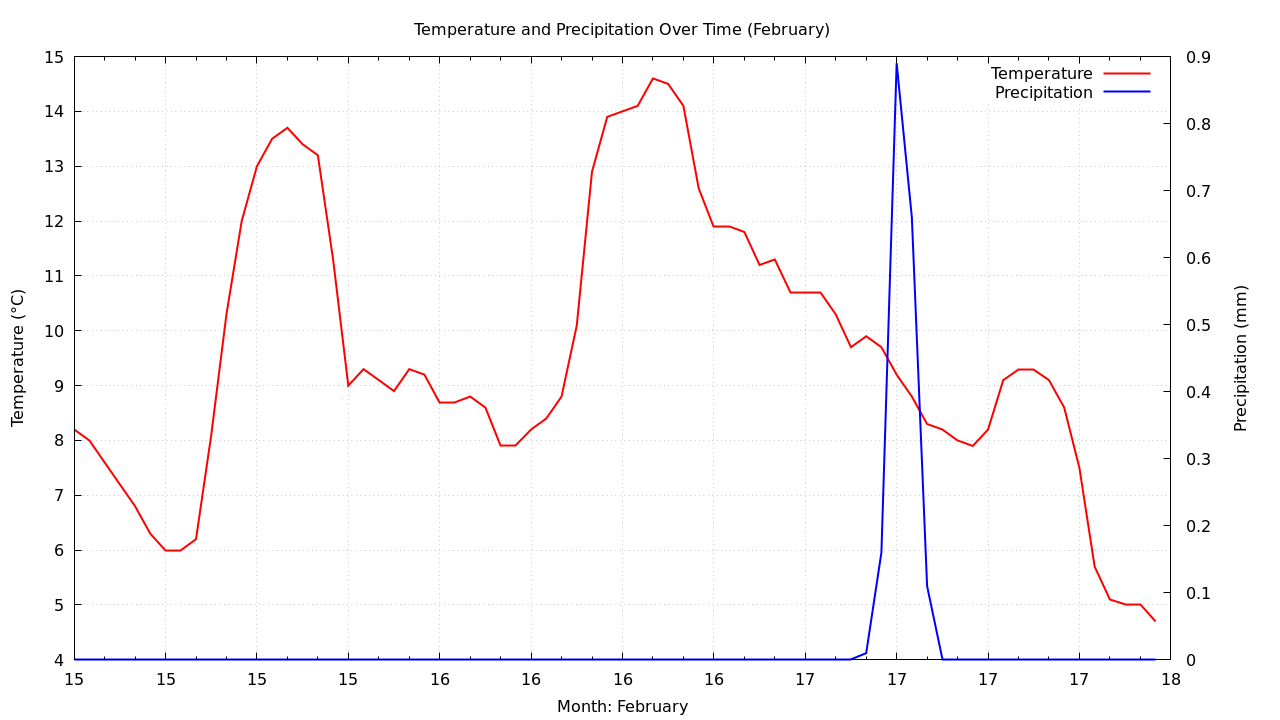
\includegraphics[width=0.8\textwidth]{data/graph/temperature_precipitation_graph.png}
\caption{Temperature and Precipitation Overview in Freiburg}
\end{figure}

\paragraph{}The following graph delves into the dynamics of wind speed, gust strength, and direction over the specified months at Freiburg. With wind speed measured in kilometers per hour, gust strength similarly quantified, and wind direction indicated in degrees, the visual representation employs distinct colors and line styles for clarity: blue signifies wind speed, green for gusts, and red indicates wind direction. This graph not only visualizes the data on a day-to-day basis but also emphasizes the variability and trends within the observed period, enriching our understanding of local wind patterns.
\begin{figure}[h]
\centering
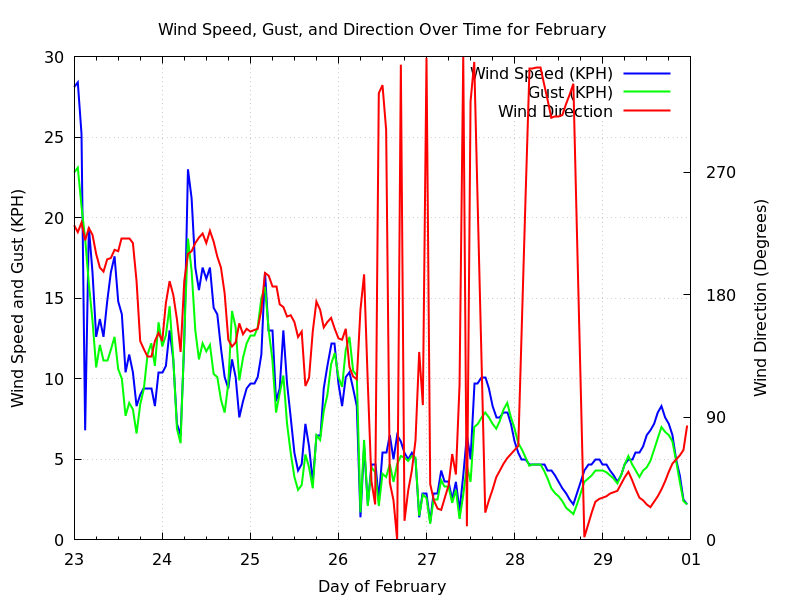
\includegraphics[width=0.8\textwidth]{data/graph/wind_speed_gust_direction_graph.png}
\caption{Detailed Wind Speed, Gust, and Direction Variations over Time in Freiburg}
\end{figure}

\paragraph{}Figure 3 presents a compelling comparison between actual and predicted weather metrics at Freiburg, including temperature, wind speed, atmospheric pressure, humidity, and visibility. Observed conditions—temperature at 5.0°C, wind speed at 9.0 kph, wind direction as 'S', pressure at 1022.0 mb, humidity at 81\%, cloud coverage at 0\%, feels like temperature at 2.9°C, and visibility at 10.0 km—are meticulously juxtaposed against their predicted counterparts. This analysis not only underscores the accuracy of weather forecasts but also reflects the intricate weather phenomena characterizing Freiburg.
\begin{figure}[h]
\centering
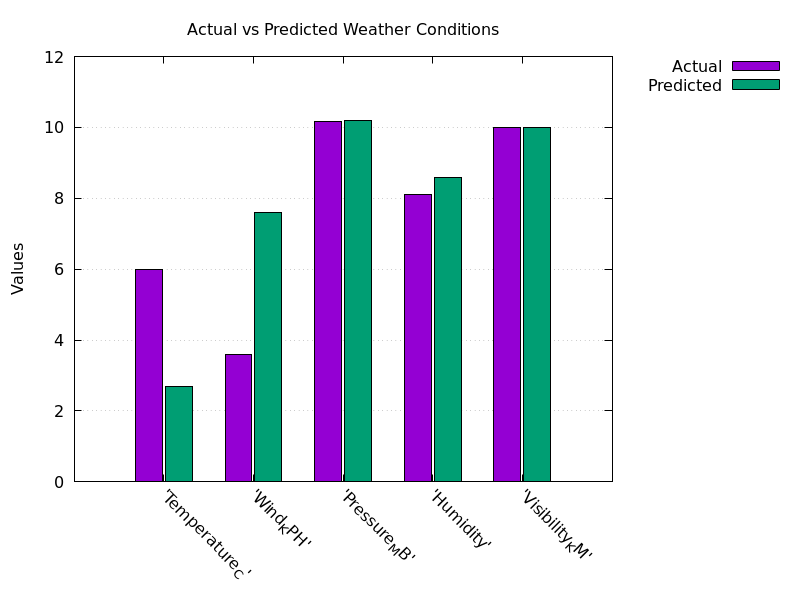
\includegraphics[width=0.8\textwidth]{data/graph/weather_comparison_graph.png}
\caption{Actual vs. Predicted Weather Conditions Analysis in Freiburg, highlighting temperature, wind speed and direction, pressure, humidity, cloud coverage, feels-like temperature, and visibility.}
\end{figure}

\end{document}